%% horizontal_self_org.tex
This chapter presents a method based on horizontal self-organisation (c.f. \secref{neuro_concepts_self_org}).
The idea of horizontal self-organisation is that the input is analysed by several smaller models instead of one big model.
This means that each network sees only a patch of the input data and cannot decide on its own what is represented in the input image, but must agree on a representation with neighbouring models.
It is important that each model is independent of the other models and that the parameters are not shared between the models. Otherwise the architecture would be comparable to vision transformer \sidecite{Dosovitskiy_Beyer_Kolesnikov_Weissenborn_Zhai_Unterthiner_Dehghani_Minderer_Heigold_Gelly_2021} and the input patches would no longer be analysed independently.


In the following, first the methodology (i.e. how horizontal self-organization is implemented) is presented and afterwards the obtained results are discussed in detail.


\section{Methods}\seclbl{horizontal_self_org_methods}
A crucial design-decision for horizontal self-organisation is the architecture of the models.
In this thesis are variational auto-encoders \sidecite{Kingma_Welling_2014} (c.f. \secref{visual_rep_learning}) used to process patches of the input image as they have a continuous latent space and are thus more robust and better interpretable (c.f. \secref{neuro_concepts_net_fragments}).

Typical auto-encoders fed an input image $\boldsymbol{x}$ through an encoder to map the input data to a latent space and through a decoder to recreate the image $\boldsymbol{\hat{x}}$. Thereby, the latent space is limited in size, forcing the model to compress the image with the encoder and to de-compress the image using the decoder.

A variational auto-encoder models the latent space as a multivariate Gaussian distribution. The input image $\boldsymbol{x}$ is also fed through a encoder and a latent representation $\boldsymbol{z}$ is obtained. Afterwards, $\boldsymbol{z}$ is fed through two independent parallel fully connected layers to obtain the $\mu$ and $\sigma$ vectors of the multivariate Gaussian distribution. Afterwards, the re-parametrization trick is used to sample a variable $\boldsymbol{z}'$ from this distribution:

\begin{equation}\eqlbl{hso_1}
	\boldsymbol{z}' \sim \mathcal{N}(\mu,\,\sigma^{2} \cdot \epsilon)
\end{equation}

$\epsilon$ is a random variable sampled from  $\mathcal{N}(0, 1)$ and determines the magnitude of the variance. The sampled latent representation is then fed through the decoder and the image $\hat{\boldsymbol{x}}$ is recreated. The model is trained to minimize a distance measure between the input image $\boldsymbol{x}$ and the reconstructed image $\hat{\boldsymbol{x}}$. In this thesis, the mean square error is used. For $n$ images $\boldsymbol{X} = \boldsymbol{x}_1, ..., \boldsymbol{x}_n$, the loss is defined as

\begin{equation}\eqlbl{hso_2}
	L_{\text{reconstruction}} = \frac{1}{n} \sum_{i=1}^{n} (\boldsymbol{x}_i - \boldsymbol{\hat{x}}_i)^2
\end{equation}

However, the latent space does not form a multivariate Gaussian distribution on the basis of this reconstruction loss and the network architecture. To accomplish this, a second loss constraint is necessary: Let $P(\boldsymbol{X})$ be the probability distribution of the data $\boldsymbol{X}$, $P(\boldsymbol{z})$ the probability distribution of the latent variable $\boldsymbol{z}$ and $P(\boldsymbol{X}|\boldsymbol{z})$ the probability distribution of generating $\boldsymbol{X}$ for a given $\boldsymbol{z}$. The objective of the VAE is to infer $P(\boldsymbol{z})$ from $P(\boldsymbol{z}|\boldsymbol{X})$ which is the probability distribution that maps $\boldsymbol{X}$ into latent space. Simply put: we want to know what the latent variable $\boldsymbol{z}$ of the input data $\boldsymbol{X}$ is.
However, $P(\boldsymbol{z}|\boldsymbol{X})$ is unknown and we have to estimate it from a simpler distribution $Q(\boldsymbol{z}|\boldsymbol{X})$. This simpler distribution $Q(\boldsymbol{z}|\boldsymbol{X})$ is learned by the encoder and should be as close as possible to the real distribution $P(\boldsymbol{z}|\boldsymbol{X})$. This is accomplished by minimizing the KL divergence\sidenote{the Kullback-Leibler (KL) divergence can ``measure'' the difference between two probability distributions} between these two probability distributions.

\begin{equation}\eqlbl{hso_3}
	KL[Q(\boldsymbol{z}|\boldsymbol{X}) || P(\boldsymbol{z}|\boldsymbol{X})] = E[\log Q(\boldsymbol{z}|\boldsymbol{X}) - \log P(\boldsymbol{z}|\boldsymbol{X})]
\end{equation}

In case of two Gaussian distributions, the KL divergence is defined as:
\begin{equation}\eqlbl{hso_4}
	KL[\mathcal{N}_Q(\mu_Q, \sigma_Q)||\mathcal{N}_P(\mu_P, \sigma_P)] = \log \frac{\sigma_P}{\sigma_Q} + \frac{\sigma_Q^2 + (\mu_Q-\mu_P)^2}{2\sigma_P^2} - \frac{1}{2}
\end{equation}


If the target distribution $P(\boldsymbol{z}|\boldsymbol{X})$ is a multivariate Gaussian distribution with $\mu_P = 0$ and $\sigma_P=1$ (i.e. $\mathcal{N}(0, 1)$) and the encoder predicts $\mu_Q$ and $\sigma_Q$ to model $Q(\boldsymbol{z}|\boldsymbol{X})$ as $\mathcal{N}(\mu_Q, \sigma_Q)$, then the KL divergence simplifies to

\begin{equation}\eqlbl{hso_5}
	\begin{align}
		KL[\mathcal{N}_Q(\mu_Q, \sigma_Q)||\mathcal{N}(0, 1)] = -\log \sigma_Q + \frac{\sigma_Q^2 \mu_Q^2}{2} - \frac{1}{2}\\
			= \frac{1}{2} (\sigma_Q^2 \mu_Q^2 - 1 - 2\log \sigma_Q)
	\end{align}
\end{equation}

Interested reads may find a formal proof of the formulas above and a more detailed derivation in the original paper \cite{Kingma_Welling_2014}.
Thus, the loss for the variational auto-encoder is defined as:











\begin{figure}[h]
    \centering
    \resizebox{0.99\textwidth}{!}
{
\begin{tikzpicture}
\tikzstyle{connection}=[ultra thick,every node/.style={sloped,allow upside down},draw=\edgecolor,opacity=0.7]
\tikzstyle{copyconnection}=[ultra thick,every node/.style={sloped,allow upside down},draw={rgb:blue,4;red,1;green,1;black,3},opacity=0.7]


\node[canvas is zy plane at x=0] (input) at (0,0,0) {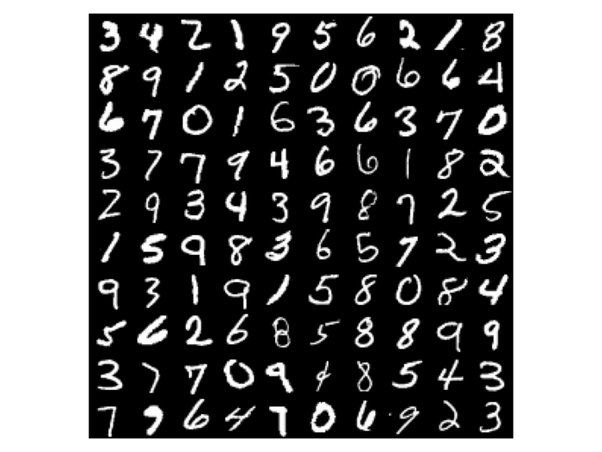
\includegraphics[width=8cm,height=8cm]{imgs/mnist.jpeg}};


\pic[shift={(3,0,0)}] at (input) 
    {Box={
        name=conv1,
        caption=Conv + ReLU,
        xlabel={{1, }},
        zlabel=32,
        fill=\ConvColor,
        height=20,
        width=2,
        depth=20
        }
    };


\draw [connection]  (input) ++(0,0,0)    -- node {\midarrow} (conv1-west);


\pic[shift={(2,0,0)}] at (conv1-east) 
    {Box={
        name=conv2,
        caption=Conv + ReLU,
        xlabel={{32, }},
        zlabel=64,
        fill=\ConvColor,
        height=12,
        width=4,
        depth=12
        }
    };


\draw [connection]  (conv1-east)    -- node {\midarrow} (conv2-west);


\pic[shift={(2,0,0)}] at (conv2-east) 
    {Box={
        name=conv3,
        caption=Conv + ReLU,
        xlabel={{64, }},
        zlabel=128,
        fill=\ConvColor,
        height=6,
        width=6,
        depth=6
        }
    };


\draw [connection]  (conv2-east)    -- node {\midarrow} (conv3-west);


\pic[shift={(2,2,0)}] at (conv3-east) 
    {Box={
        name=fcn1,
        caption=FC + ReLU,
        xlabel={{" ","dummy"}},
        zlabel=32,
        fill=\SoftmaxColor,
        opacity=0.8,
        height=3,
        width=3,
        depth=6
        }
    };


\pic[shift={(2,-2,0)}] at (conv3-east) 
    {Box={
        name=fcn2,
        caption=FC + ReLU,
        xlabel={{" ","dummy"}},
        zlabel=32,
        fill=\SoftmaxColor,
        opacity=0.8,
        height=3,
        width=3,
        depth=6
        }
    };


\draw [connection]  (conv3-east)    -- node {\midarrow} (fcn1-west);


\draw [connection]  (conv3-east)    -- node {\midarrow} (fcn2-west);


\pic[shift={(2,-2,0)}] at (fcn1-east) 
    {Box={
        name=conv4,
        caption=Conv + ReLU,
        xlabel={{128, }},
        zlabel=64,
        fill=\ConvColor,
        height=6,
        width=6,
        depth=6
        }
    };


\draw [connection]  (fcn1-east)    -- node {\midarrow} (conv4-west);


\draw [connection]  (fcn2-east)    -- node {\midarrow} (conv4-west);


\pic[shift={(2,0,0)}] at (conv4-east) 
    {Box={
        name=conv5,
        caption=Conv + ReLU,
        xlabel={{64, }},
        zlabel=32,
        fill=\ConvColor,
        height=12,
        width=4,
        depth=12
        }
    };


\draw [connection]  (conv4-east)    -- node {\midarrow} (conv5-west);


\pic[shift={(2,0,0)}] at (conv5-east) 
    {Box={
        name=conv6,
        caption=Conv + ReLU,
        xlabel={{32, }},
        zlabel=1,
        fill=\ConvColor,
        height=20,
        width=2,
        depth=20
        }
    };


\draw [connection]  (conv5-east)    -- node {\midarrow} (conv6-west);


\node[canvas is zy plane at x=3] (output) at (conv6-east) {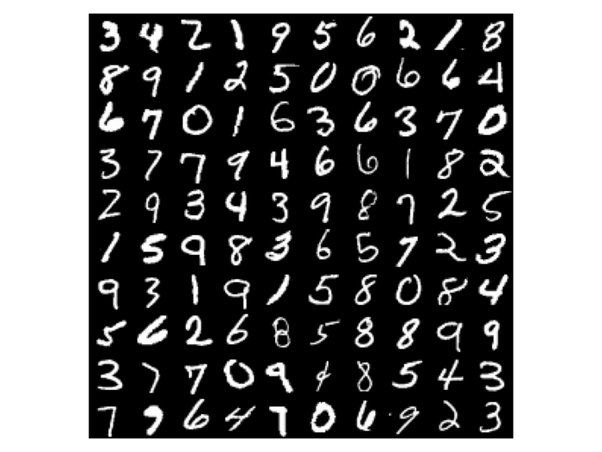
\includegraphics[width=8cm,height=8cm]{imgs/mnist.jpeg}};


\draw [connection]  (conv6-east)     -- node {\midarrow} ($(output) + (0.5,0,0)$);


\end{tikzpicture}
}
    \caption[Architecture of the variational auto-encoder used for horizontal self-organisation]{Architecture of the variational auto-encoder used for horizontal self-organisation.}
    \figlbl{horizontal_org_arch1}
\end{figure}

\section{Results}\seclbl{horizontal_self_org_results}










%TODO: vereinheitliche Mathe: Was ist underline, was ist hochgestellt in Klammern ($z^{(i)}$) und was ist hochgestellt in eckigen Klammern? Bei NN: Was ist n, was ist m, ... (+ Lernraten Symbol, Loss Symbol, etc.)
%Sind alle Vektoren bold?

% TODO: target function und objective function vereinheitlichen
% TODO: net-fragment or net fragment

